\section{Conceptos generales}

\subsection{Definición de un fluido}
Un fluido es una sustancia que siempre se deforma continuamente cuando se somete a un esfuerzo cortante, sin importar qué tan pequeño sea dicho esfuerzo.\\

Tiene \textbf{propiedades} que lo caracterizan y definen el estado en el que se encuentra, pudiendo determinar su comportamiento. Algunas de estas propiedades son: \\
\begin{center}
	\begin{tabular} {r l}
		Densidad & $\rho = \dfrac{m}{V} \;[kg/m^3]$ \\
		Viscosidad & $\mu \;[kg/m s]$ \\
		Peso & $P \;[kgf] [N]$\\
		Peso específico & $\gamma \;[kgf/m^3]$ \\
		Temperatura & $T \;[°C]$ \\
	\end{tabular}
\end{center}

A fines de simplificar cálculos, consideramos la densidad de un fluido constante.

También consideramos la estructura molecular de los fluidos como \emph{continuo}, esto quiere decir que las propiedades de este varían en forma continua a lo largo de su estructura o se mantienen constantes.


\subsection{Ecuación de Newton para los fluidos}
Para obtener la ecuación de newton para los fluidos, se plantea un sistema en el que un fluido se entra entre dos placas paralelas separadas por una cierta distancia, como se muestra en la figura \ref{fig:fluido-placas-paralelas}. La placa inferior es fija y a la superior se le aplica una fuerza $F$ lo que produce un esfuerzo cortante en el fluido, y a su vez establece una velocidad en la placa superior.

Si la fuerza $F$, por más pequeña que sea, hace que la placa se mueva permanentemente, entonces la sustancia es un fluido.

\begin{figure}[H]
	\centering
	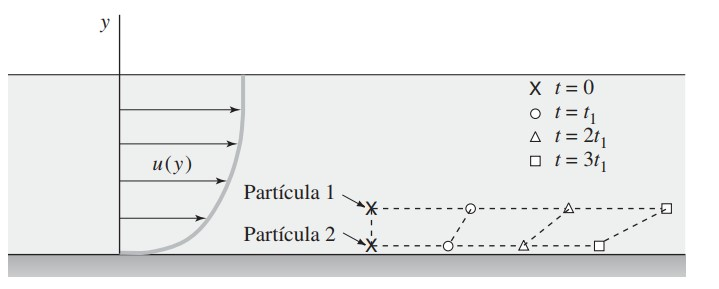
\includegraphics[width = .8\linewidth]{cortante3}
	\caption{Movimiento relativo de dos partículas de fluido en presencia de esfuerzos cortantes}
	\label{fig:fluido-placas-paralelas}
 \end{figure}

Manteniendo ciertas cantidades constantes, como la viscosidad $\mu$ del fluido, el area de las placas, la distancia entre ellas y la velocidad de la placa superior, se llega a una expresión que relaciona la fuerza aplicada con los parámetros mencionados:
\begin{equation}
	F = \mu \dfrac{A \cdot U}{y}
	\label{eq:fuerza}
\end{equation}

Considerando que el esfuerzo se calcula como la fuerza aplicada en un área:

\begin{equation*}
	\tau = \dfrac{F}{A}
	\label{eq:esfuerzo}
\end{equation*}

y reemplazando a la fuerza $F$ por la expresión \ref{eq:fuerza} se llega a la ecuación para determinar el esfuerzo cortante en función de la viscosidad, la velocidad del fluido y la altura:

\begin{equation}
	\tau = \mu \dfrac{U}{y} \hspace{.3cm};\hspace{.3cm} \tau = \mu \dfrac{du}{dy}
\end{equation}

El término $\dfrac{du}{dy}$ es un gradiente de velocidad y puede ser interpretada como una \textbf{velocidad de deformación}.\\ 


A partir de esta definición, los fluidos se pueden clasificar como \textit{newtonianos} o \textit{no newtonianos}.

\subsubsection{Fluidos newtonianos}

Los fluidos newtonianos son aquellos fluidos donde su viscosidad es constante, es decir, la relación entre el esfuerzo cortante y de velocidad de deformación es lineal, como se muestra en la figura \ref{diag:fluido-newtoniano}.



\begin{figure}[H]
	\centering
	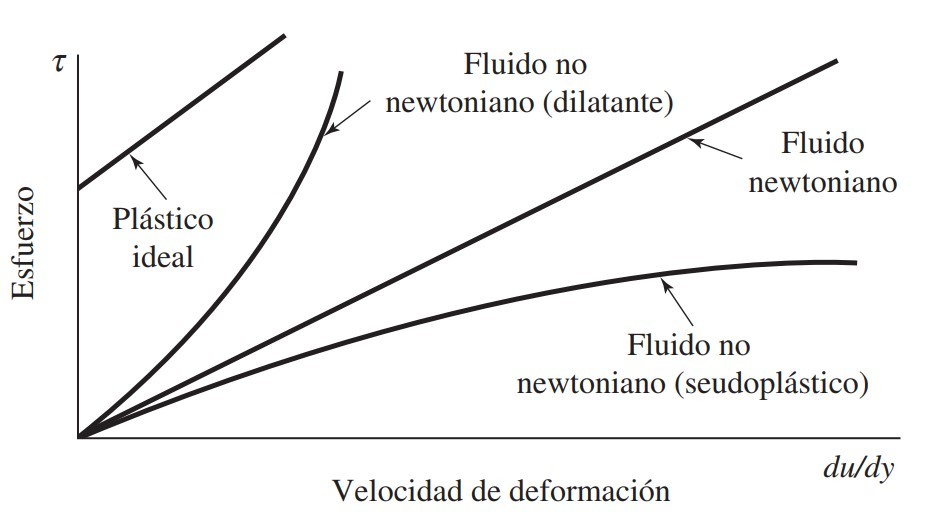
\includegraphics[width= .7\linewidth]{tipo-fluido}
	\caption{Fluidos newtonianos y no newtonianos}
	\label{diag:fluido-newtoniano}
\end{figure}

\subsubsection{Fluidos ideales}

Un fluido ideal se considera cuando su viscosidad es nula, por lo tanto el esfuerzo cortante requerido será nulo sin importar su movimiento.

En la figura \ref{diag:fluido-newtoniano} un fluido ideal se representaría como una recta vertical que atraviesa el origen de coordenadas.



\subsection{Viscosidad}
\subsubsection{Viscosidad absoluta o dinámica $\mu$}
La viscosidad es una propiedad propia del fluido e indica el grado de resistencia a los esfuerzos cortantes.

En los gases, la viscosidad absoluta incrementa con la temperatura, en cambio, en los líquidos disminuye junto con esta. 

En un líquido, esto se debe directamente a la cohesión entre las moléculas de la sustancia. Esta disminuye cuando aumenta la temperatura. En cambio en gases, la viscosidad se debe por el movimiento aleatorio de las moléculas, y éste aumenta con la temperatura.

\subsubsection{Viscosidad cinemática $v$}

Es la relación entre la viscosidad absoluta y la densidad de la sustancia
\begin{equation}
	v = \dfrac{\mu}{\rho}
\end{equation}

\subsection{Compresibilidad y tensión superficial}
\subsubsection{Compresibilidad}
La compresibilidad es la capacidad de un fluido de disminuir su volumen bajo la aplicación de una presión. Los gases son altamente compresibles mientra que los líquidos, muy poco. 

En la materia \materia se trabaja con fluidos ideales no compresibles, es decir, de viscosidad cero.\\

\subsubsection{Tensión superficial}

El fenómeno de tensión superficial se debe a las fuerzas de cohesión y adhesión entre las partículas. Sobre la superficie del liquido las fuerzas cohesivas desde abajo exceden a las fuerzas adhesivas desde el gas localizado por encima del fluido (figura \ref{fuerzas_cohesivas_adhesivas}), dando como resultado una tensión superficial.

\begin{figure}[h]
	\centering
	\begin{subfigure}[b]{.45\linewidth}
		\centering
		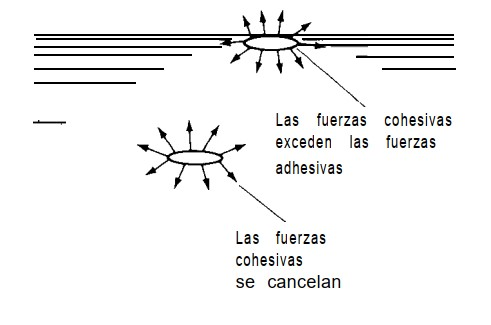
\includegraphics[width = .7\linewidth]{fuerzas}
		\caption{Fuerzas cohesivas y adhesivas}
		\label{fuerzas_cohesivas_adhesivas}
	\end{subfigure}
	\begin{subfigure}[b]{.45\linewidth}
		\centering
		\begin{subfigure}[b]{.45\linewidth}
			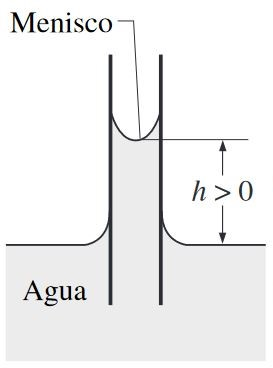
\includegraphics[width = .7\linewidth]{efecto-capilar-agua}
			\caption{}
			\label{fig:capilaridad-agua}
		\end{subfigure}
		\begin{subfigure}[b]{.45\linewidth}
			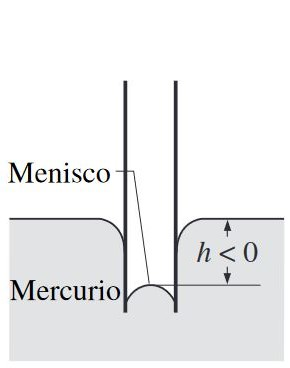
\includegraphics[width = .7\linewidth]{efecto-capilar-mercurio}
			\caption{}
			\label{fig:capilaridad-mercurio}
		\end{subfigure}
	\end{subfigure}
	\caption{Tensión superficial}
\end{figure}

En el caso de un líquido que se encuentra en contacto con un sólido, si la adhesión del líquido con el sólido es mayor que la cohesión en el líquido mismo, entonces éste \emph{subirá} dentro del tubo y formará con el sólido un menisco curvado hacia arriba, como muestra la figura \ref{fig:capilaridad-agua}. Puede pasar también que las fuerzas de adhesión sean menores que las de cohesión y entonces el menisco estará curvado hacia abajo, como el caso del mercurio y el vidrio en la figura \ref{fig:capilaridad-mercurio}.\\ %Ver para agregar la figura del mercurio, entoces queda más copado si se puede ver el efecto.

Podemos calcular la altura h que se desplaza el fluido igualando la componente vertical de la fuerza de tensión superficial (que actúa en la dirección $\theta$) con el peso de la columna de fluido, como:
%Agregar una imagen del esquema, si es que hay una, entonces no queda al aire el planteo

\begin{equation*}
	\sigma \pi \cos \beta = \gamma \dfrac{\pi D^2}{4} h
\end{equation*}
\begin{equation}
	h = \dfrac{4 \sigma \cos \beta}{\gamma D}
\end{equation}

donde $\sigma$ es la tensión superficial.

\subsection{Presión de vapor}
Cuando un liquido se evapora, las moléculas escapan desde la superficie líquida.  Si el espacio por encima del líquido se encuentra confinado, el equilibrio se logrará cuando el número de moléculas de vapor que se condensan es igual al número de moléculas que escapan de la superficie. La presión resultante de las moléculas de vapor se conoce como \emph{presión de vapor} y es directamente proporcional a la temperatura. Cuando la presión por encima del líquido iguala a la presión de vapor de este, se produce la ebullición. \\

En flujos líquidos, pueden crearse condiciones que lleven la presión por debajo de la presión de vapor del líquido. Cuando ocurre esto se forman burbujas localmente, fenómeno llamado \emph{cavitación}.



